\section{Introduction to Security and Cryptology}

\subsection{Cryptography Fundamentals}

\begin{definition}{Cryptography Goals}
    Cryptography aims to achieve four fundamental security properties:
    \begin{itemize}
        \item \textbf{Confidentiality} - Information is only accessible to authorized parties
        \item \textbf{Integrity} - Information has not been altered in an unauthorized way
        \item \textbf{Authenticity} - Origin of information can be verified
        \item \textbf{Freshness/Non-repudiation} - Information is current and sender cannot deny transmission
    \end{itemize}
    These goals align with the broader CIA triad of information security but add authentication and non-repudiation.
\end{definition}


\subsubsection{Model der Kommunikation und Verschlüsselung}

\begin{definition}{Kommunikationsmodel}

    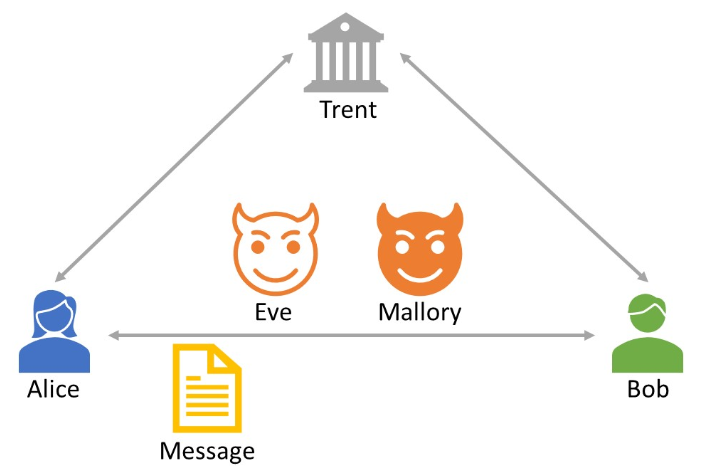
\includegraphics[width=0.7\linewidth]{kommunikationsmodel.png}

    \begin{itemize}
        \item \textcolor{darkblue}{\textbf{Alice}} sendet eine Nachricht an Bob. Dabei sollen die oben genannten Ziele, confidentiality, integrity, authenticity, non-repudiation und freshness erfüllt werden.
        \item \textcolor{darkgreen}{\textbf{Bob}} empfängt die Nachrichten von Allice. Er will überprüfen können, dass die Ziele eingehalten wurden.
        \item \textcolor{darktangerine}{\textbf{Eve}}  ist ein Attacker. Sie kann Nachrichten mitlesen, aber sie nicht verändern.
        \item \textcolor{darkred}{\textbf{Mallory}} ist ein anderer Attacker. Er kann Daten sowohl mitlesen als auch verändern. Er kann auch Nachrichten abfangen und später weitersenden, oder ganz verwerfen. Er kann auch neue Nachrichten generieren.
        \item \textcolor{darkgrey}{\textbf{Trent}} ist eine Drittperson/Instanz, welcher sowohl Alice und Bob vertrauen. Trent unterstützt Alice und Bob bei der sicheren Kommunikation.
    \end{itemize}
\end{definition}

\begin{concept}{Model der Verschlüsselung}
    Um eine vertrauliche Kommunikation zu erreichen, werden Nachrichten vor dem Senden verschlüsselt und nach dem Empfangen wieder entschlüsselt.

    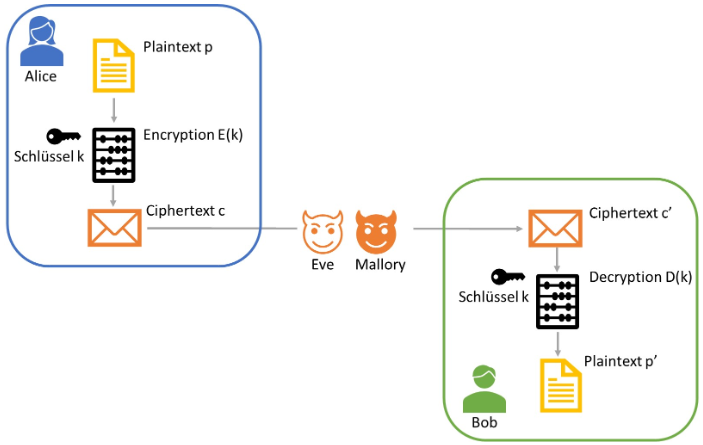
\includegraphics[width=\linewidth]{model_der_verschluesselung.png}

    \begin{itemize}
        \item \textcolor{darkcorn}{\textbf{Plaintext (Klartext):}} Der Plaintext ist der Text, so wie er geschrieben, respektive gelesen werden kann. Er wird mit dem Buchstaben "p" abgekürzt.
        \item \textcolor{darkorange}{\textbf{Ciphertext (Verschlüsselter Text):}} Der Ciphertext ist der Text, welcher durch die Verschlüsselung entsteht. Er wird mit dem Buchstaben "c" abgekürzt.
        \item \textcolor{darkturquoise}{\textbf{Encryption (Verschlüsselung):}} Die Verschlüsselung macht aus dem Plaintext den dazugehörenden Ciphertext. Dazu wird ein Schlüssel verwendet. Die Verschlüsselung kann wie folgt angegeben werden: $c=E[k](p)$. Der Verschlüsselungsalgorithmus selbst ist öffentlich bekannt und kann von allen analysiert werden, um mögliche Schwachstellen zu finden.
        \item \textcolor{darkturquoise}{\textbf{Decryption (Entschlüsselung):}} Die Entschlüsselung macht aus einem Ciphertext den dazugehörenden Plaintext. Dazu wird ein Schlüssel verwendet. Die Entschlüsselung kann wie folgt angegeben werden p' = D[k](c'). Der Entschlüsselungsmechanismus ist öffentlich bekannt und kann von allen analysiert werden, um mögliche Schwachstellen zu finden.
        \item \textcolor{darkpink}{\textbf{Key (Schlüssel):}} Nur mit dem richtigen Schlüssel, kann eine Nachricht richtig entschlüsselt werden. Je nach Art der Verschlüsselung wird derselbe Key für die Verschlüsselung und die Entschlüsselung verwendet (Secret Key Kryptographie) oder es werden unterschiedliche Schlüssel verwendet (Public Key Kryptographie). Damit die Verschlüsselung sicher ist, muss der Schlüssel, welcher für die Entschlüsselung gebraucht wird, geheim bleiben.
    \end{itemize}    
\end{concept}

\subsection{Encryption and Properties}

\begin{concept}{Encryption}
    Encryption is a transformation from P (plaintexts) to C (ciphertexts) under control of some key, chosen from K (key space).
    
    The idea is to have a whole family of transformations, where each key gives a different transformation.
    \begin{itemize}
        \item $c = E(k, p) = E_k(p)$
        \item $p = D(k, c) = D_k(c)$
    \end{itemize}
    
    Each transformation must be reversible. It follows that $|C|$ can not be smaller than $|P|$. In fact most often we have $P = C$.
\end{concept}

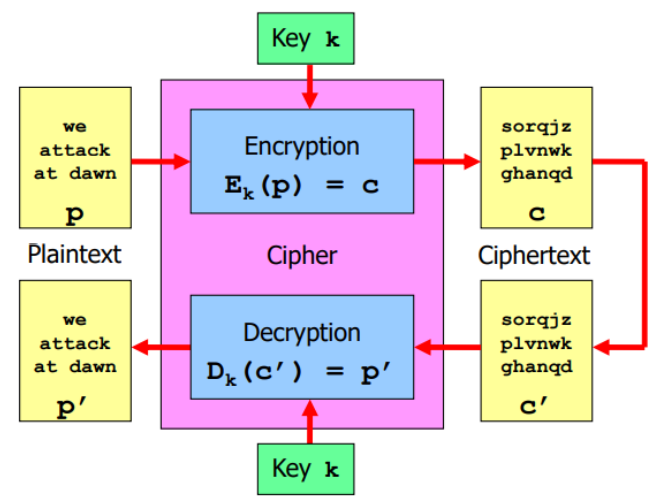
\includegraphics[width=0.6\linewidth]{encryption_decryption.png}

\subsubsection{Attacktypen auf Kryptosysteme}

\begin{remark}
    Die Unterschiede zwischen den Attacken bestehen daraus, auf was der Attacker Zugriff hat.
\end{remark}

\begin{definition}{Ciphertext-only attack}
    Der Attacker kann vom Ciphertext alleine Rückschlüsse auf den Plaintext oder den 
    verwendeten Schlüssel ziehen.
\end{definition}

\begin{definition}{Chosen-ciphertext attack}
    Der Attacker kann Ciphertexte generieren und diese vom System entschlüsseln lassen. 
    Der Attacker bekommt entweder den zum gewählten Ciphertext gehörenden Plaintext 
    (und kann daraus potenziell Rückschlüsse auf den verwendeten Schlüssel machen) 
    oder er bekommt nur Teilinformationen, wie zum Beispiel 
    "Die Entschlüsselung konnte / konnte nicht durchgeführt werden".
\end{definition}

\begin{definition}{Known-plaintext attack}
    Der Attacker kennt sowohl Teile des Plaintext als auch den dazugehörenden Ciphertext (oder zumindest Teile davon). 
    Er kann daraus Rückschlüsse auf andere Plaintexte oder gar den Schlüssel machen.
\end{definition}

\begin{definition}{Chosen-plaintext attack}
    Der Attacker kann Plaintexte wählen, welche er vom System verschlüsseln lassen will. 
    Er erhält dann den dazugehörenden Ciphertext und kann daraus Rückschlüsse auf 
    andere Plaintexte oder gar den Schlüssel machen.
\end{definition}

\begin{definition}{Brute-force attack}
    Der Attacker probiert alle möglichen Schlüssel aus, bis er den richtigen gefunden hat. 
    Dass er den richtigen gefunden hat, erkennt er daran, dass der erhaltene Plaintext sinnvoll erscheint.
\end{definition}

\begin{remark}
    Grundsätzlich können alle Verschlüsselungsalgorithmen mittels brute-force Attacken geknackt werden. 
    Ein wichtiges Evaluationskriterium eines Verschlüsselungsalgorithmus ist also, wie lange eine solche brute-force Attacke im Durchschnitt benötigt. Dieser Anzahl sagt man auch kryptographischer Work Factor.
\end{remark}

\raggedcolumns
\columnbreak

\subsection{Cryptographic Work Factor}

\begin{definition}{Work Factor}
    The number of times it takes to come upon the correct key is called (cryptographic) work factor.
    \begin{itemize}
        \item Work factor (WF) = average number of keys to try
        \item Work factor is usually given in bits: $\log_2(n)$, $n = key\ space\ size$
    \end{itemize}
\end{definition}

\begin{formula}{Entropy}
    Entropy is maximal if all outcomes are equally likely
    $$H = \sum_{i=1}^{n} p(i) \cdot \log_2 \left(\frac{1}{p(i)}\right)$$
    
    $$H_{binary} = \sum_{i=1}^{n} \frac{1}{n} \log_2(n) = \log_2(n)$$
\end{formula}

\begin{concept}{Entropy of Cryptographic Keys}\\
    Cryptographic keys are typically created with random generators, so they can be considered as elements of a random variable.
    
    What's the entropy of a key with 128-bit?
    \begin{itemize}
        \item Independent with equal probability: $128 \cdot 1 = 128$ bits
        \item Dependent with inequal probability: $p(0) = 0.25, p(1) = 0.75 \rightarrow 128 \cdot 0.81 \approx 104$ bits
    \end{itemize}
\end{concept}

\begin{theorem}{Relation between entropy and work factor}\\
    Work Factor $\approx$ entropy, key size = max. entropy $\approx$ max. work factor
\end{theorem}

\subsection{Security Models}

\begin{definition}{Information-theoretically secure}
    Intercepting a ciphertext tells you nothing about the plain
\end{definition}

\begin{definition}{Computationally secure}
    Work factor $\approx$ key entropy
\end{definition}

\subsection{Secret Key Cryptography}

\subsubsection{Perfect Secrecy and One-Time Pad}

\begin{theorem}{Perfect Secrecy}
    A cryptographic system has perfect secrecy if for all possible plaintexts $p$ and ciphertexts $c$:
    \begin{equation}
        P[p|c] = P[p]
    \end{equation}
    This means that observing the ciphertext provides no information about the plaintext.
\end{theorem}

\begin{concept}{One-Time Pad (Vernam Cipher)}
    The only known encryption scheme with perfect secrecy:
    \begin{itemize}
        \item Key must be completely random and at least as long as the message
        \item Encryption: $c_j = p_j \oplus k_j$ for all bits $j$
        \item Each key can only be used once
        \item If reused: $P_1 \oplus P_2 = C_1 \oplus C_2$ (major vulnerability)
    \end{itemize}
    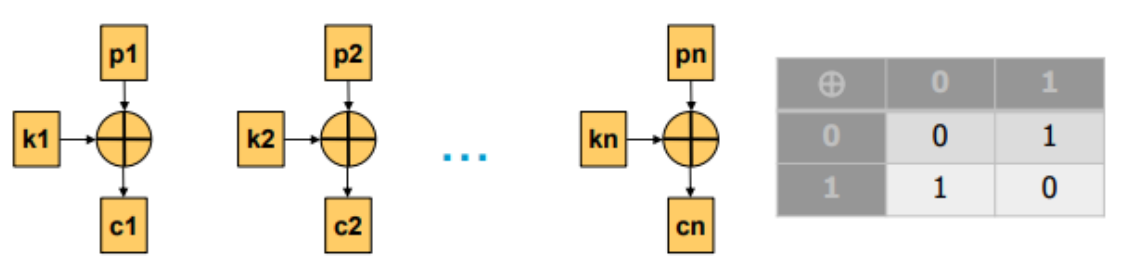
\includegraphics[width=0.7\linewidth]{vernam_cipher.png}
\end{concept}

\begin{concept}{Limitations of One-Time Pad}
    Despite perfect security, OTP is rarely used due to practical limitations:
    \begin{itemize}
        \item Key must be as long as the message
        \item Key must be completely random
        \item Key must be pre-shared securely
        \item Key can only be used once
    \end{itemize}
\end{concept}

\subsubsection{Modern Symmetric Encryption}

\begin{concept}{Modern Cipher Properties}
    Since perfect secrecy is impractical, modern ciphers aim for computational security:
    \begin{itemize}
        \item Publicly known algorithms
        \item No known practical attacks
        \item Work factor > $2^{128}$
        \item Use standardized implementations only
    \end{itemize}
\end{concept}

\begin{concept}{Block Ciphers}
    Block ciphers encrypt fixed-size blocks of data:
    \begin{itemize}
        \item Require padding for messages not multiple of block size
        \item Use modes of operation for longer messages (ECB, CBC, CTR, GCM)
        \item Examples: DES (insecure), Triple-DES (legacy), AES (current standard)
    \end{itemize}
    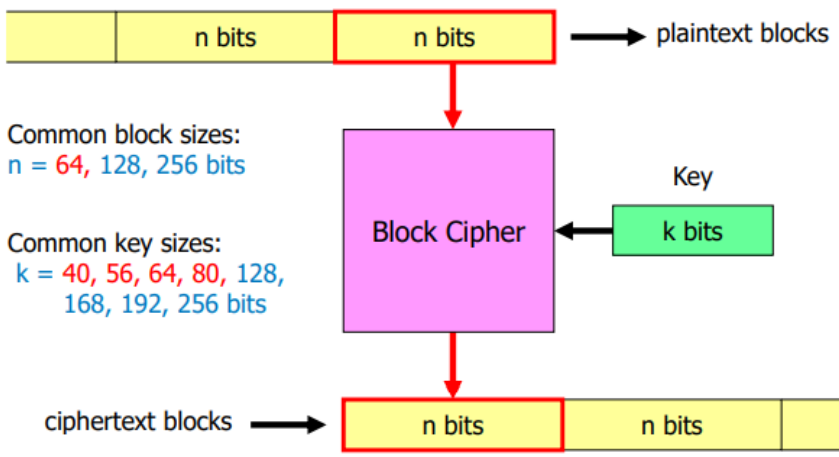
\includegraphics[width=\linewidth]{block_cipher.png}
\end{concept}

\begin{concept}{Stream Ciphers}
    Stream ciphers encrypt data bit-by-bit or byte-by-byte:
    \begin{itemize}
        \item No need to wait for complete blocks
        \item Generally faster than block ciphers
        \item Most historical stream ciphers are broken (RC4, A5/1, A5/2)
        \item ChaCha20 is the current standard for stream ciphers
    \end{itemize}
    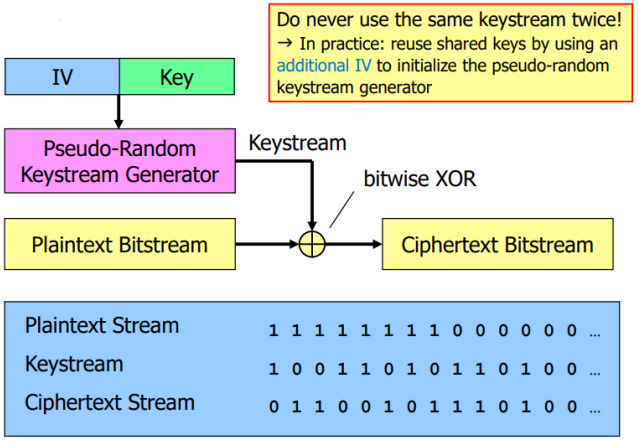
\includegraphics[width=\linewidth]{stream_ciphers.png}
\end{concept}

\subsection{Public Key Cryptography}

\subsubsection{Key Distribution Problem}

\begin{concept}{Key Distribution Challenge}
    Secret key cryptography faces significant scalability issues:
    \begin{itemize}
        \item Keys must be exchanged securely before communication
        \item Difficult to establish keys with unknown parties
        \item $n$ users require $\frac{n(n-1)}{2}$ key pairs for complete connectivity
        \item Key management complexity grows quadratically
    \end{itemize}
    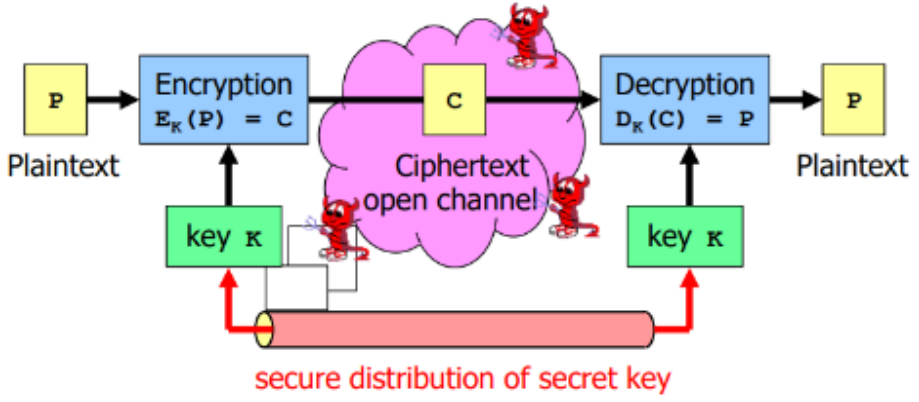
\includegraphics[width=0.5\linewidth]{key_distribution.png}
\end{concept}

\subsubsection{Public Key Principles}

\begin{definition}{Public Key Cryptography}
    Uses mathematically related key pairs for encryption and decryption:
    \begin{itemize}
        \item \textbf{Public Key} - Known to everyone, used for encryption
        \item \textbf{Private Key} - Known only to owner, used for decryption
        \item Keys are mathematically related: $D(E(M)) = M$
        \item Private key cannot be feasibly computed from public key
    \end{itemize}
    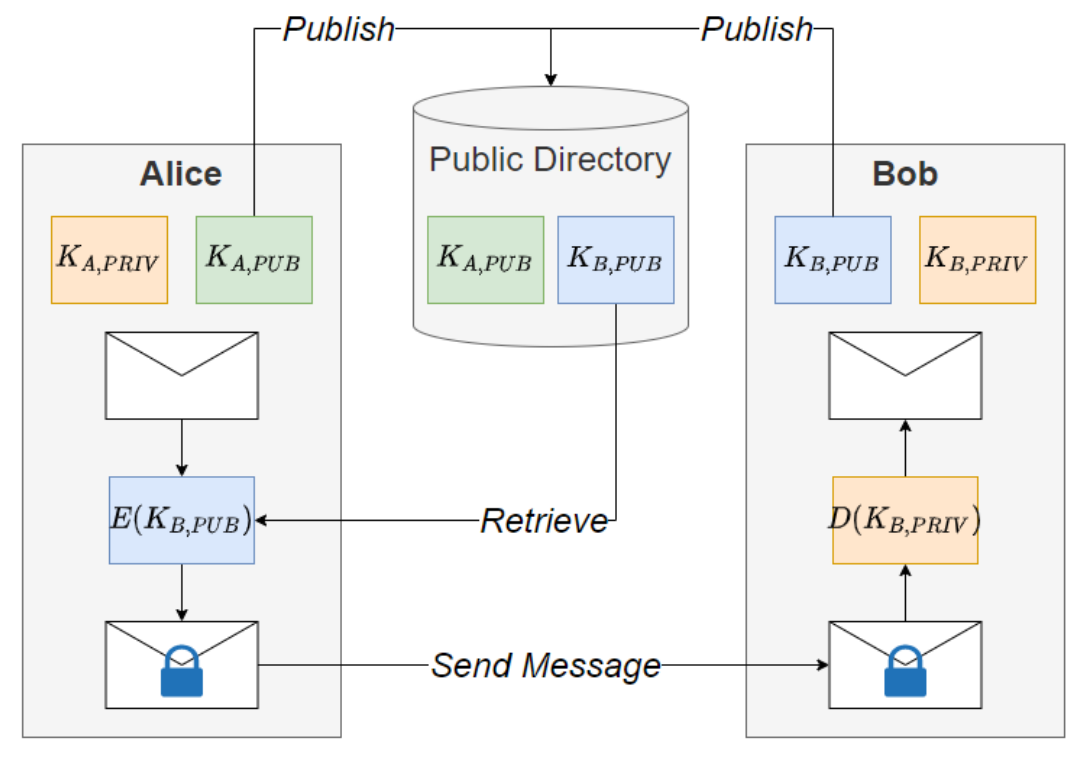
\includegraphics[width=\linewidth]{public_key.png}
\end{definition}

\subsubsection{RSA Algorithm}

\begin{definition}{RSA Cryptosystem}
    Based on the computational difficulty of factoring large numbers:
    \begin{itemize}
        \item Public Key: $(n, e)$ where $n = p \cdot q$ (product of large primes)
        \item Private Key: $(n, d)$ where $ed \equiv 1 \pmod{\varphi(n)}$
        \item Encryption: $c = m^e \bmod n$
        \item Decryption: $m = c^d \bmod n$
    \end{itemize}
\end{definition}

\subsubsection{Diffie-Hellman Key Exchange}

\begin{KR}{Diffie-Hellman Protocol}
    \paragraph{Setup}
    Alice and Bob agree on public parameters:
    \begin{itemize}
        \item Large prime $p$
        \item Generator $g$ of the multiplicative group $\mathbb{Z}_p^*$
    \end{itemize}
    
    \paragraph{Key Generation}
    \begin{itemize}
        \item Alice chooses private $a$, computes $A = g^a \bmod p$
        \item Bob chooses private $b$, computes $B = g^b \bmod p$
        \item They exchange $A$ and $B$ publicly
        \item Shared secret: $S = B^a = A^b = g^{ab} \bmod p$
    \end{itemize}
    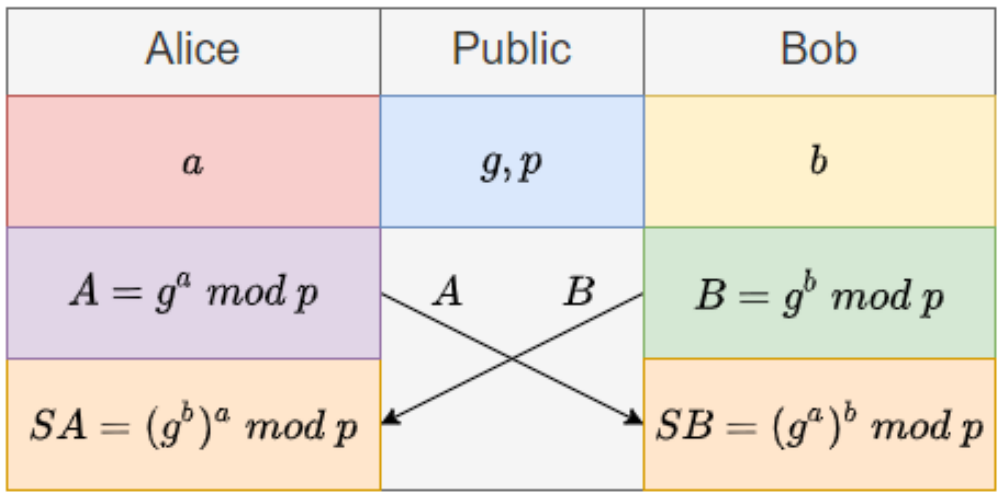
\includegraphics[width=\linewidth]{diffie_hellman_diagram.png}
\end{KR}

\subsection{Hash Functions and Message Authentication}

\subsubsection{Cryptographic Hash Functions}

\begin{definition}{Cryptographic Hash Function}
    A function that takes arbitrary-length input and produces fixed-length output:
    \begin{itemize}
        \item \textbf{Efficient computation} - Fast to compute
        \item \textbf{Preimage resistance} - Hard to find input for given output
        \item \textbf{Collision resistance} - Hard to find two inputs with same output
        \item \textbf{Pseudo-random output} - Small input changes cause large output changes
    \end{itemize}
\end{definition}

\subsubsection{Message Authentication Codes}

\begin{definition}{Message Authentication Code (MAC)}
    Combines hash functions with secret keys for message integrity:
    \begin{itemize}
        \item Detects unauthorized message modifications
        \item Provides authentication of message origin
        \item Requires shared secret key between sender and receiver
        \item HMAC is the most common MAC construction
    \end{itemize}
    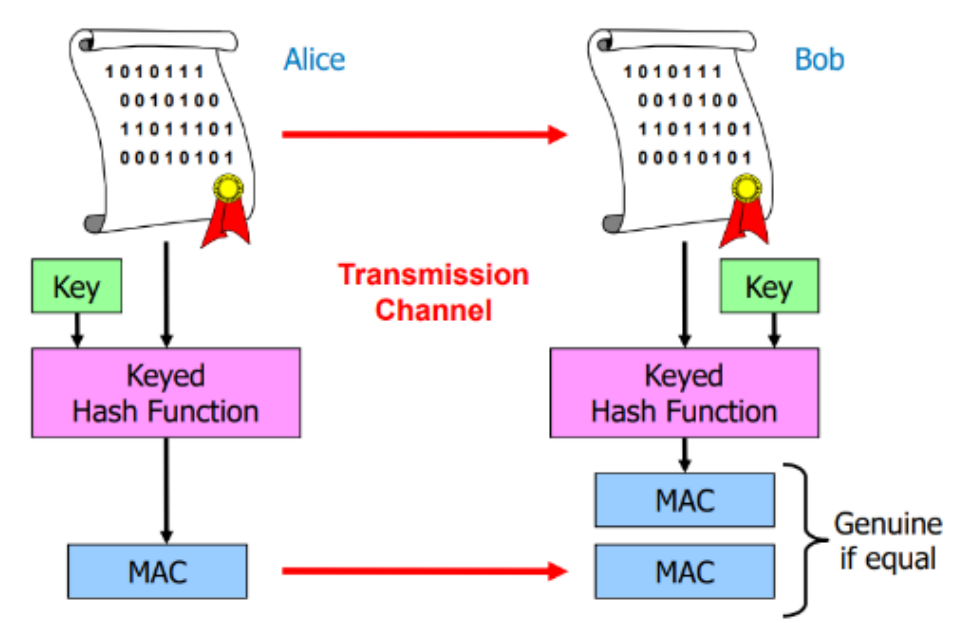
\includegraphics[width=0.8\linewidth]{MAC.png}
\end{definition}

\begin{concept}{HMAC Construction}
    Hash-based Message Authentication Code:
    \begin{itemize}
        \item $\text{HMAC}(K, M) = H((K \oplus \text{opad}) || H((K \oplus \text{ipad}) || M))$
        \item Uses nested hash function calls with key padding
        \item Secure when used with cryptographic hash functions
        \item Resistant to length extension attacks
    \end{itemize}
    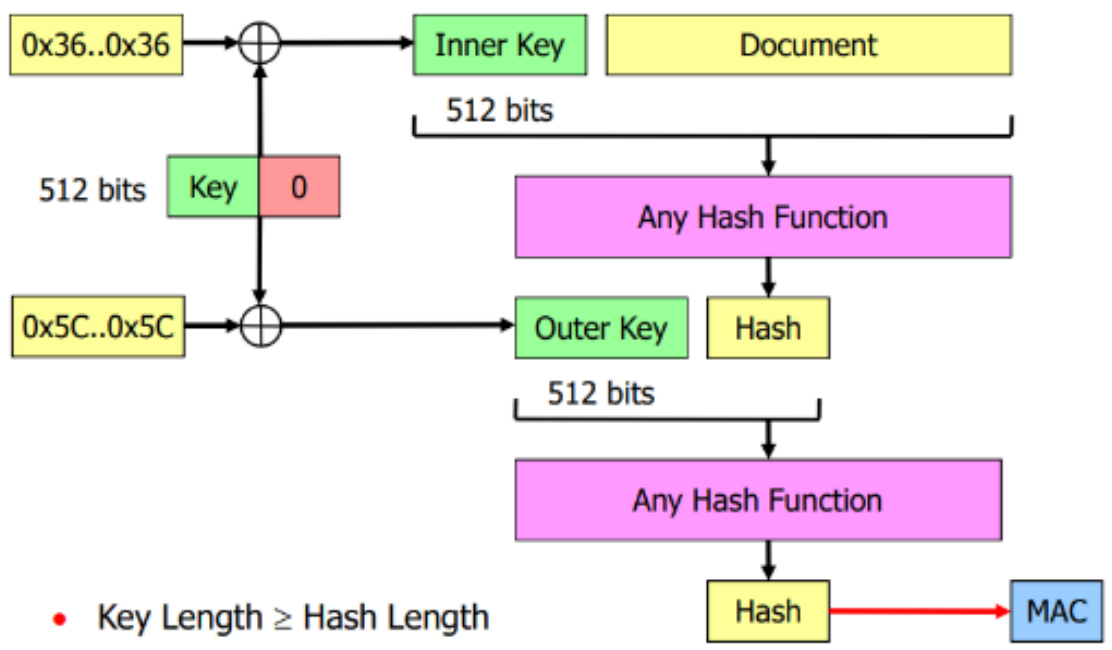
\includegraphics[width=\linewidth]{HMAC.png}
\end{concept}

\subsubsection{Digital Signatures}

\begin{concept}{Digital Signatures vs. MACs}
    \begin{itemize}
        \item \textbf{MACs}: Fast, require shared secret, provide authentication
        \item \textbf{Digital Signatures}: Slower, use public keys, provide non-repudiation
        \item Signatures enable verification by anyone with the public key
        \item MACs only verifiable by parties with the shared secret
    \end{itemize}
    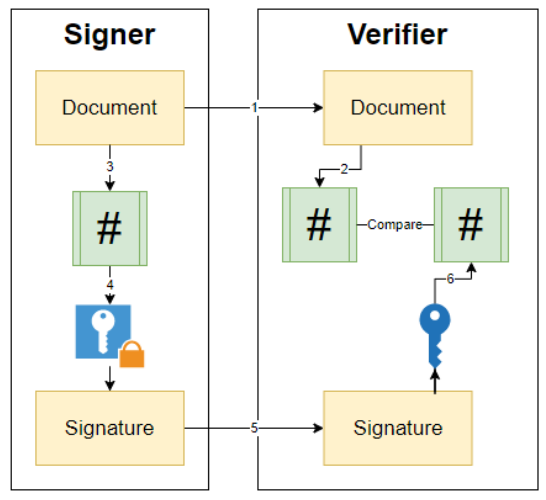
\includegraphics[width=0.8\linewidth]{digital_signature.png}
\end{concept}

\subsubsection{Authenticated Encryption}

\begin{concept}{Galois Counter Mode (GCM)}
    Combines encryption and authentication in a single operation:
    \begin{itemize}
        \item Provides both confidentiality and integrity protection
        \item Uses counter mode encryption with Galois field authentication
        \item Widely supported in TLS and other protocols
        \item Efficient implementation in hardware and software
    \end{itemize}
    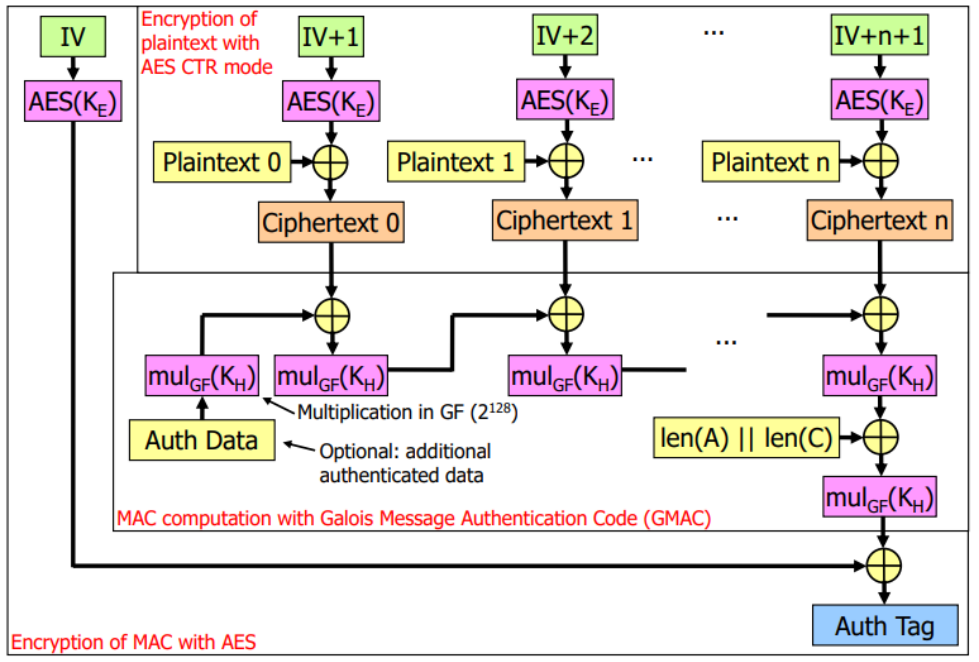
\includegraphics[width=0.8\linewidth]{GCM.png}
\end{concept}


